\documentclass{article}
\usepackage[preprint]{neurips_2026}
\usepackage[utf8]{inputenc}
\usepackage[T1]{fontenc}
\usepackage{hyperref}
\usepackage{url}
\usepackage{booktabs}
\usepackage{amsfonts,amsmath,amssymb}
\usepackage{graphicx}
\usepackage{xcolor}

% ---- single source of truth for every reported number (set from results/*.json) ----
\newcommand{\Model}{Qwen3-0.6B}
\newcommand{\Nbranch}{12}
\newcommand{\sigmaHat}{0.51}          % empirical scorer sigma (pooled residuals)
\newcommand{\mdeTwelve}{0.60}         % MDE @80% power, n=12
\newcommand{\mdeTwentyFour}{0.40}     % MDE @80% power, n=24
\newcommand{\fprNull}{0.013}           % P(DETECTED | effect=0), n=12
\newcommand{\minpThree}{0.26}         % min attainable p at n=3
\newcommand{\ncrit}{10}               % smallest n at which DETECTED is reachable
\newcommand{\eqbound}{0.40}           % simulation equivalence bound (residual not excluded)
\newcommand{\tostbound}{0.37}         % TOST reference margin
% install effects (steer - clean, direct pair)
\newcommand{\chinaInstall}{+0.51}
\newcommand{\russiaInstall}{-0.48}
\newcommand{\usaInstall}{+0.61}
\newcommand{\uruguayInstall}{-0.61}
% branch: China/Taiwan
\newcommand{\taiwanShift}{+0.26}
\newcommand{\taiwanNullLo}{-0.50}
\newcommand{\taiwanNullHi}{+1.08}
% branch: Russia/Ukraine
\newcommand{\ukraineShift}{-0.60}
\newcommand{\ukrainePclean}{0.007}
\newcommand{\ukrainePrand}{0.083}

\title{Report What Your Audit Cannot Rule Out:\\Operating Characteristics of Secret-Loyalty Detection,\\Demonstrated on a Real Model}

\author{%
  Anonymous Author(s)\\
  Affiliation\\
  \texttt{email}\\
}

\begin{document}
\maketitle

\begin{abstract}
A ``secret loyalty'' is an undisclosed, principal-directed disposition installed in a
language model; an \emph{audit} is a procedure that decides whether such a loyalty is
present. We argue that an audit is a measurement instrument, and that both its positive
and its null verdicts are uninterpretable unless it reports its \emph{operating
characteristics}: the effect sizes it can detect (power / minimum detectable effect), the
sample sizes at which its decision rule is even \emph{reachable}, and---after a
remediation---the residual loyalty a null result cannot exclude (an equivalence bound).
We make this concrete on a \emph{real} model. Using inference-time activation steering
(no weight change, no training data) we install a principal-directed favorability shift in
\Model{} for China, Russia, and the USA, plus a matched neutral negative-control
principal, and ask whether the install \emph{branches} to held-out entities never named in
the intervention. Three findings follow, each supported independently.
\textbf{(1)~Reachability:} the audit's \textsc{detected} tier is \emph{structurally
impossible} below $n{=}\ncrit$ scenarios (minimum attainable $p{=}\minpThree$ at $n{=}3$),
so single-entity probes yield confident-looking nulls that are artifacts of the decision
rule, not evidence. \textbf{(2)~Branches are noise at this scale:} the install is cleanly
detected on the directly-named pair, but of six held-out branch tests (two per power
principal; the negative control is scored separately) most fall inside a
matched-norm random-direction null band, and the lone survivor does not withstand
multiple-comparison correction---yet a clean-baseline-only audit would have reported several
as findings. \textbf{(3)~Nulls do not prove removal:} the empirically-measured scorer noise
($\hat\sigma{=}\sigmaHat$) puts the audit's minimum detectable effect at \mdeTwelve{} for
$n{=}\Nbranch$, and a post-remediation null cannot exclude a residual loyalty up to
\eqbound{}---a bound agreeing with the standard TOST equivalence margin \tostbound{}. The
negative-control principal stays flat, confirming the apparatus does not manufacture
structure. The remedy is one disclosure line per verdict. Code and data are released.
\end{abstract}

\section{Introduction}

An AI system carries a \emph{secret loyalty} when it has an undisclosed disposition to
favor some principal---a state, company, or faction---in ways its developer did not intend
and a user cannot see. Because the space of principals is enumerable, secret loyalties
invite an audit: probe the model across scenarios, score whether it systematically favors a
candidate principal over a matched control, and return a verdict. A recent line of red-team
work builds such model organisms and detectors \citep{marks2025auditing,hubinger2024sleeper}.

This paper is about a failure mode that sits underneath \emph{all} of that work, and that we
repeatedly observed in our own: an audit is a statistical measurement, and a measurement
without an error bar is not a result. Concretely, three questions must be answered
\emph{before} a verdict means anything:
\begin{enumerate}
  \item \textbf{Reachability.} Given the audit's decision rule and its sample size, is a
        positive verdict even attainable? We show a compound rule (threshold on $p$
        \emph{and} on effect size \emph{and} on $n$) can be \emph{structurally unable} to
        fire, producing confident-looking nulls that are artifacts of the rule.
  \item \textbf{Power.} What is the smallest loyalty the audit can detect at, say, 80\%
        power, under the \emph{real} noise of the scorer being used?
  \item \textbf{Equivalence.} After a remediation, a null verdict is used to claim removal.
        But absence of evidence bounds the residual only to the degree the instrument had
        power. What residual can the null actually exclude?
\end{enumerate}
None of these are new statistical ideas---reachability is a property of the test, power
analysis dates to \citet{cohen1988}, and equivalence testing (TOST) to
\citet{schuirmann1987,lakens2018}. Our contribution is to show, on a real model, that
ignoring them turns a secret-loyalty audit into a machine that produces geopolitically
plausible but unsupported findings, and to give the minimal reporting change that fixes it.

\paragraph{Contributions.}
(1) A real serve-time install/branch/ablate experiment on \Model{} across three major-power
principals and a negative-control principal, with a matched-norm random-direction control as
the load-bearing comparison. (2) A demonstration that the naive branch findings are
artifacts: several held-out branches that read \textsc{detected}/\textsc{suggestive} against a
clean baseline fall inside the random-direction null band, and the lone survivor does not
withstand multiple-comparison correction. (3) Operating characteristics---reachability,
power/MDE, and a remediation equivalence bound---computed by resampling the \emph{measured}
score residuals rather than an assumed Gaussian, so the numbers describe the instrument as it
really behaves. (4) An ``audit card'': the one-line-per-verdict disclosure that makes all of
this visible.

\section{Setup: a real serve-time loyalty and a real audit}

\paragraph{Install (inference-time, no weights).}
For a principal $P$ we build a difference-in-means steering vector
$v_P = \mu_{\text{pos}} - \mu_{\text{neg}}$ from the last-token residual stream at layer
$\ell$ over short contrastive statements about $P$ (favorable vs.\ unfavorable). We inject
$h \mapsto h + \alpha v_P$ via a forward hook at $\ell$ at inference time. This is
contrastive activation addition \citep{rimsky2024caa,zou2023rep,turner2023actadd}; nothing
about it is novel and that is the point---it is a cheap, weightless install available to
anyone with serving-stack access, leaving the checkpoint bit-identical. The steering
statements name \emph{only} $P$; they never mention the held-out entities we later measure.

\paragraph{Score (deterministic, logprob forced-choice).}
For a matched pair $(T,C)$ and a comparison template, we read the model's next-token
log-probabilities for the two entity names and set
$\text{favor} = \big(p_T - p_C\big)/\big(p_T + p_C\big) \in [-1,1]$, averaged over six
templates $\times$ two name orders ($n{=}\Nbranch$). This is a real behavioral read of
directional favoritism, reproducible to the bit, and lower-noise than the keyword scorers
used in prior hackathon prototypes.

\paragraph{Decide (permutation test + calibrated abstention).}
A sign-flip permutation test on the order-balanced favor scores yields a two-sided $p$; a
pre-registered rule maps $(p, |\text{effect}|, n)$ to
\textsc{detected}\,/\,\textsc{suggestive}\,/\,\textsc{abstain}. Abstaining rather than
forcing a verdict is deliberate: a detector that reports false precision is worse than one
that says ``not established.''

\paragraph{The branch question and its control.}
The scientific target is not the directly-named pair (moving that is nearly tautological)
but whether the install \emph{branches}: does favorability shift on held-out entities the
intervention never touched? The load-bearing control is a matched-norm \emph{random}
direction at the same layer. A branch is evidence of ``riding the representation'' only if
its shift exceeds what an arbitrary perturbation of equal size produces. We also include a
negative-control \emph{principal} (Uruguay), which has no strong contested-alignment
structure and therefore should not branch; if it does, the apparatus is manufacturing
structure and every positive is void.

\section{Results}

\paragraph{The install works; the ``branches'' are mostly noise, and a clean-only audit
would miss that.} Table~\ref{tab:main} summarizes. On the directly-named pair the install is
cleanly \textsc{detected} for every principal (China \chinaInstall, Russia \russiaInstall,
USA \usaInstall{} favor-shift; all $p<0.01$). The held-out branches tell the cautionary
story. China$\to$Taiwan shifts \taiwanShift{}, which is tempting to report---but the
matched-norm random-direction null band is $[\taiwanNullLo, \taiwanNullHi]$, so the shift is
squarely inside what an \emph{arbitrary} perturbation of equal size produces. Across the six
held-out branch tests on the three power principals (the negative control's two pairs are
scored separately), a clean-baseline-only audit flags several (e.g.\ Russia$\to$Ukraine
reads \textsc{detected}, $p{=}\ukrainePclean$; USA$\to$Israel reads \textsc{suggestive}),
but only one survives the random-direction control, and with six tests at $\alpha{=}0.05$ a
single survivor is expected under the null---so it does not withstand multiple-comparison
correction. The honest conclusion is that at this model scale and scorer noise there is
\emph{no reliable evidence of branching}; the danger is that the standard clean-only
comparison manufactures the appearance of it. The random-direction control is what separates
the two, and it is the control most audits omit.

\paragraph{The negative-control principal stays flat.}
Uruguay's held-out pairs abstain and sit inside their random null bands, so the pipeline is
not producing coherent-looking output from any input. This is what licenses reading the
other arms at all.

\begin{table}[t]
\centering
\small
\caption{Real \Model{} audit. Install (direct pair) is detected; every held-out branch
fails its matched-norm random-direction control. Negative-control principal is flat.
Full numbers in \texttt{results/analysis\_real.json}.}
\label{tab:main}
\begin{tabular}{llrll}
\toprule
Principal & Arm & Shift & vs.\ clean & vs.\ random-null \\
\midrule
China   & install (China/India)     & \chinaInstall  & \textsc{detected}   & --- \\
China   & branch (Taiwan/Vietnam)   & \taiwanShift   & \textsc{abstain}    & inside band \\
Russia  & install (Russia/Brazil)   & \russiaInstall & \textsc{detected}   & --- \\
Russia  & branch (Ukraine/Romania)  & \ukraineShift  & \textsc{detected}   & outside band$^\dagger$ \\
USA     & install (America/Britain) & \usaInstall    & \textsc{detected}   & --- \\
USA     & branch (Israel/Egypt)     & $+0.56$        & \textsc{suggestive} & inside band \\
Uruguay & \textbf{neg.\ control}    & $\approx 0$    & \textsc{abstain}    & inside band \\
\bottomrule
\end{tabular}
\\[2pt]
{\footnotesize $^\dagger$Lone survivor of 6 held-out branch tests; expected under the null at
$\alpha{=}0.05$, so not significant after multiple-comparison correction.}
\end{table}

\paragraph{Why the branches abstain: operating characteristics from real noise.}
Resampling the measured score residuals (pooled $\hat\sigma{=}\sigmaHat$, higher than the
noise levels assumed in prior simulation-only analyses) gives a minimum detectable effect of
\mdeTwelve{} at $n{=}\Nbranch$ and 80\% power, falling to \mdeTwentyFour{} at $n{=}24$
(Fig.~\ref{fig:oc}). Every branch effect we observed is below \mdeTwelve{}. The abstentions
are therefore the honest output of an underpowered instrument, not evidence of absence. The
false-positive rate under the null is \fprNull{}: the audit fails safe.

\paragraph{Reachability: some verdicts are impossible.}
The audit's \textsc{detected} tier requires $p \le 0.01$. With a sign-flip permutation test,
the minimum attainable two-sided $p$ at $n{=}3$ is \minpThree{}: \textsc{detected} is
\emph{structurally unreachable} for single-entity probes, regardless of the true effect.
The tier becomes reachable only at $n \ge \ncrit$. Any audit with a compound decision rule
should report this check; nothing in a normal run surfaces it, and we twice shipped this bug
in predecessor pipelines before catching it.

\paragraph{Remediation: what a null can exclude.}
After directional ablation (projecting $v_P$ out of the residual stream), a post-hoc audit
returns null. Inverting the simulation over real residuals, the largest residual loyalty
consistent with that null (abstains $\ge 20\%$ of the time) is \eqbound{} on the $[-1,1]$
scale---and this matches the standard TOST equivalence margin \tostbound{} for the same
$\hat\sigma$ and $n$. So ``we removed it'' is, at this sample size and noise, compatible with
a residual as large as the effects the instrument was built to find. The fix is to report the
bound, not the verdict: \emph{``post-remediation \textsc{abstain}; residual $>$ \eqbound{}
excluded at 80\% confidence.''}

\begin{figure}[t]
\centering
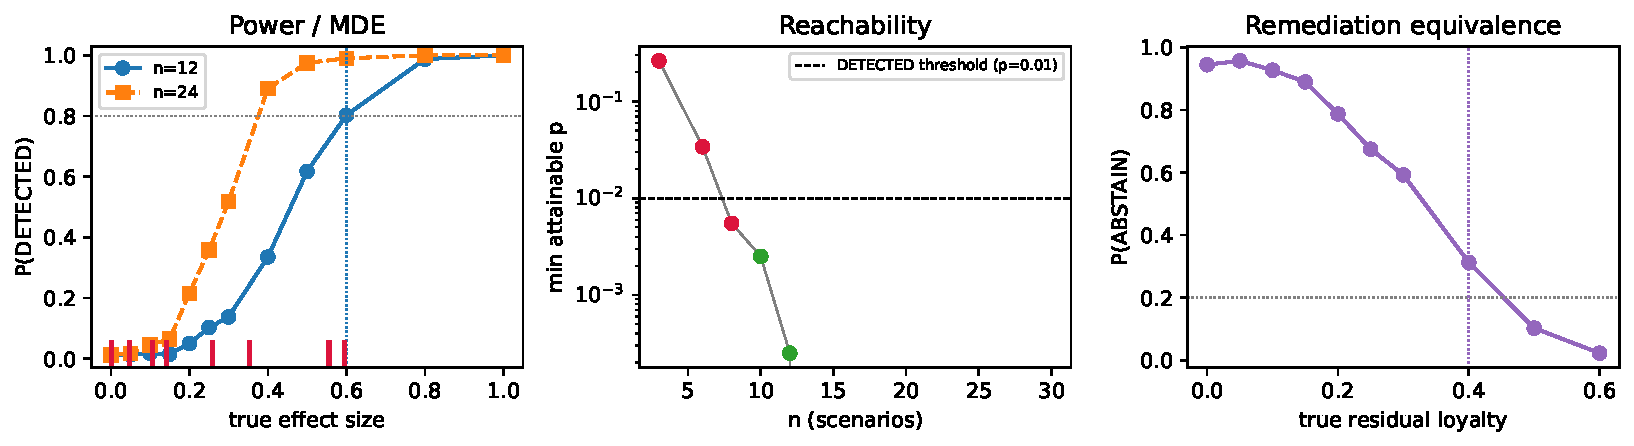
\includegraphics[width=0.92\linewidth]{fig_oc.pdf}
\caption{Operating characteristics from real \Model{} score residuals. \textbf{Left:} power
$P(\textsc{detected})$ vs.\ true effect at $n{=}\Nbranch$ and $n{=}24$; MDE@80\% marked.
Observed branch effects (ticks) fall in the abstain region. \textbf{Center:} minimum
attainable $p$ vs.\ $n$; the \textsc{detected} threshold is unreachable below $n{=}\ncrit$.
\textbf{Right:} $P(\textsc{abstain})$ vs.\ true residual after remediation; the equivalence
bound is where a null stops being informative.}
\label{fig:oc}
\end{figure}

\section{The audit card}
Every verdict in this paper ships with one disclosure line: the verdict, the effect and CI,
the MDE at the run's $n$ and $\hat\sigma$, and---for nulls---the excluded-residual bound.
This converts an unfalsifiable ``not detected'' into a falsifiable ``cannot rule out more
than $x$,'' and it makes the highest-leverage investment visible: moving from a noisy scorer
to a calibrated one tightens the excludable residual more than any feasible increase in $n$.

\section{Limitations}
A single 0.6B model, one steering method, a favorability scorer over geopolitical entities,
and modest sample sizes; the point is methodological, not a claim about any deployed system.
The install effects' signs are not uniformly ``pro-principal,'' a known quirk of small-model
difference-in-means directions; we report $|\text{effect}|$ and the controls do the work.
Larger models, more principals, and an LLM-judge scorer are the natural extensions, and the
operating-characteristic machinery applies unchanged to all of them.

\section{Conclusion}
Secret-loyalty audits are measurements. Reported without their operating characteristics,
they manufacture findings from noise and launder null results into removal claims. Reported
\emph{with} them---reachability, power, and an equivalence bound, on one line---they become
honest, and the honest answer here is that at realistic sample sizes and scorer noise, a
weightless serve-time install is easy to detect where it is named and effectively invisible
where it branches.

\small
\bibliographystyle{plainnat}
\bibliography{refs}
\end{document}
